\documentclass[]{article}
\usepackage[T1]{fontenc}
\usepackage{lmodern}
\usepackage{amssymb,amsmath}
\usepackage{ifxetex,ifluatex}
\usepackage{fixltx2e} % provides \textsubscript
% use upquote if available, for straight quotes in verbatim environments
\IfFileExists{upquote.sty}{\usepackage{upquote}}{}
\ifnum 0\ifxetex 1\fi\ifluatex 1\fi=0 % if pdftex
  \usepackage[utf8]{inputenc}
\else % if luatex or xelatex
  \ifxetex
    \usepackage{mathspec}
    \usepackage{xltxtra,xunicode}
  \else
    \usepackage{fontspec}
  \fi
  \defaultfontfeatures{Mapping=tex-text,Scale=MatchLowercase}
  \newcommand{\euro}{€}
\fi
% use microtype if available
\IfFileExists{microtype.sty}{\usepackage{microtype}}{}
\usepackage[margin=1in]{geometry}
\usepackage{color}
\usepackage{fancyvrb}
\newcommand{\VerbBar}{|}
\newcommand{\VERB}{\Verb[commandchars=\\\{\}]}
\DefineVerbatimEnvironment{Highlighting}{Verbatim}{commandchars=\\\{\}}
% Add ',fontsize=\small' for more characters per line
\usepackage{framed}
\definecolor{shadecolor}{RGB}{248,248,248}
\newenvironment{Shaded}{\begin{snugshade}}{\end{snugshade}}
\newcommand{\KeywordTok}[1]{\textcolor[rgb]{0.13,0.29,0.53}{\textbf{{#1}}}}
\newcommand{\DataTypeTok}[1]{\textcolor[rgb]{0.13,0.29,0.53}{{#1}}}
\newcommand{\DecValTok}[1]{\textcolor[rgb]{0.00,0.00,0.81}{{#1}}}
\newcommand{\BaseNTok}[1]{\textcolor[rgb]{0.00,0.00,0.81}{{#1}}}
\newcommand{\FloatTok}[1]{\textcolor[rgb]{0.00,0.00,0.81}{{#1}}}
\newcommand{\CharTok}[1]{\textcolor[rgb]{0.31,0.60,0.02}{{#1}}}
\newcommand{\StringTok}[1]{\textcolor[rgb]{0.31,0.60,0.02}{{#1}}}
\newcommand{\CommentTok}[1]{\textcolor[rgb]{0.56,0.35,0.01}{\textit{{#1}}}}
\newcommand{\OtherTok}[1]{\textcolor[rgb]{0.56,0.35,0.01}{{#1}}}
\newcommand{\AlertTok}[1]{\textcolor[rgb]{0.94,0.16,0.16}{{#1}}}
\newcommand{\FunctionTok}[1]{\textcolor[rgb]{0.00,0.00,0.00}{{#1}}}
\newcommand{\RegionMarkerTok}[1]{{#1}}
\newcommand{\ErrorTok}[1]{\textbf{{#1}}}
\newcommand{\NormalTok}[1]{{#1}}
\usepackage{graphicx}
% Redefine \includegraphics so that, unless explicit options are
% given, the image width will not exceed the width of the page.
% Images get their normal width if they fit onto the page, but
% are scaled down if they would overflow the margins.
\makeatletter
\def\ScaleIfNeeded{%
  \ifdim\Gin@nat@width>\linewidth
    \linewidth
  \else
    \Gin@nat@width
  \fi
}
\makeatother
\let\Oldincludegraphics\includegraphics
{%
 \catcode`\@=11\relax%
 \gdef\includegraphics{\@ifnextchar[{\Oldincludegraphics}{\Oldincludegraphics[width=\ScaleIfNeeded]}}%
}%
\ifxetex
  \usepackage[setpagesize=false, % page size defined by xetex
              unicode=false, % unicode breaks when used with xetex
              xetex]{hyperref}
\else
  \usepackage[unicode=true]{hyperref}
\fi
\hypersetup{breaklinks=true,
            bookmarks=true,
            pdfauthor={Jacques Botes},
            pdftitle={Statistical Inference: Exponential Distribution Simulation},
            colorlinks=true,
            citecolor=blue,
            urlcolor=blue,
            linkcolor=magenta,
            pdfborder={0 0 0}}
\urlstyle{same}  % don't use monospace font for urls
\setlength{\parindent}{0pt}
\setlength{\parskip}{6pt plus 2pt minus 1pt}
\setlength{\emergencystretch}{3em}  % prevent overfull lines
\setcounter{secnumdepth}{0}

\title{Statistical Inference: Exponential Distribution Simulation}
\author{Jacques Botes}
\date{September 2014}

\begin{document}

\begin{center}
\huge Statistical Inference: Exponential Distribution Simulation \\[0.2cm]
\end{center}
\begin{center}
\large \emph{Jacques Botes}\\[0.1cm]
\end{center}
\begin{center}
\large \emph{September 2014} \\
\end{center}
\normalsize


\begin{verbatim}
## Loading required package: ggplot2
\end{verbatim}

\subsection{Problem Statement}\label{problem-statement}

The exponential distribution can be simulated in R with
\texttt{rexp(n, lambda)} where lambda is the rate parameter. The mean of
exponential distribution is 1/lambda and the standard deviation is also
also 1/lambda. Set lambda = 0.2 for all of the simulations. In this
simulation, you will investigate the distribution of averages of 40
exponential(0.2)s. Note that you will need to do a thousand or so
simulated averages of 40 exponentials.

\begin{enumerate}
\def\labelenumi{\arabic{enumi}.}
\itemsep1pt\parskip0pt\parsep0pt
\item
  Show where the distribution is centered at and compare it to the
  theoretical center of the distribution.
\item
  Show how variable it is and compare it to the theoretical variance of
  the distribution.
\item
  Show that the distribution is approximately normal.
\item
  Evaluate the coverage of the confidence interval for
  $1/\lambda = \bar{X} \pm 1.96 \frac{S}{\sqrt{n}}$.
\end{enumerate}

First setup the simulation and get the means of the 1000 simulations

\begin{Shaded}
\begin{Highlighting}[]
\KeywordTok{set.seed}\NormalTok{(}\DecValTok{9867}\NormalTok{)}
\NormalTok{n <-}\StringTok{ }\DecValTok{1000}        \NormalTok{## no of runs}
\NormalTok{sample.size <-}\StringTok{ }\DecValTok{40} \NormalTok{## 40 samples in each run}
\NormalTok{lambda <-}\StringTok{ }\FloatTok{0.2}   \NormalTok{##variable input}
\NormalTok{dist <-}\StringTok{ }\KeywordTok{matrix}\NormalTok{(}\KeywordTok{rexp}\NormalTok{(sample.size*n, }\DataTypeTok{rate=}\NormalTok{lambda), }\DataTypeTok{ncol =} \NormalTok{sample.size, }\DataTypeTok{nrow=}\NormalTok{n)}
\NormalTok{dist.means <-}\StringTok{ }\KeywordTok{rowMeans}\NormalTok{(dist) ##a  vector of n length with averages in each row based on sample size means}
\end{Highlighting}
\end{Shaded}

\begin{enumerate}
\def\labelenumi{\arabic{enumi}.}
\itemsep1pt\parskip0pt\parsep0pt
\item
  Show where the distribution is centered at and compare it to the
  theoretical center of the distribution.
  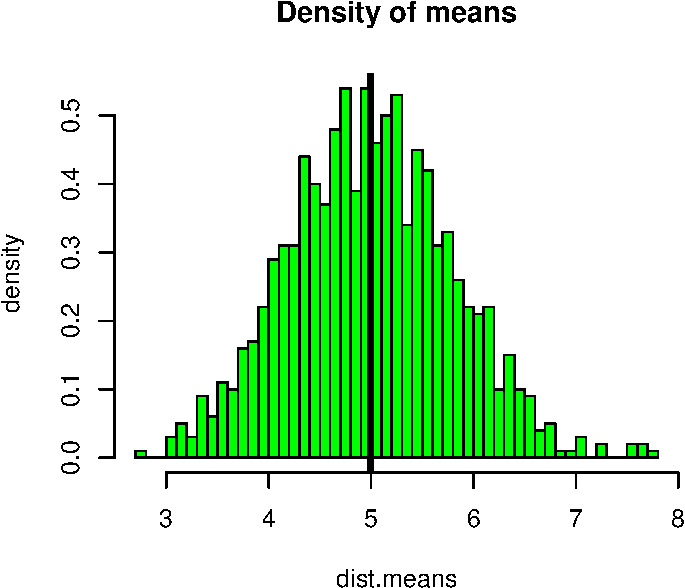
\includegraphics{./Q1_files/figure-latex/Q1.pdf}
\end{enumerate}

The Theoretical center of the distribution is calculated as $1/\lambda$
= 1/0.2 = 5. The center of the distribution is 4.9951. The black line in
the above plot displays the center.

\begin{enumerate}
\def\labelenumi{\arabic{enumi}.}
\setcounter{enumi}{1}
\itemsep1pt\parskip0pt\parsep0pt
\item
  Show how variable it is and compare it to the theoretical variance of
  the distribution.
\end{enumerate}

\begin{Shaded}
\begin{Highlighting}[]
\NormalTok{sd.ac <-}\StringTok{ }\KeywordTok{sd}\NormalTok{(dist.means)}
\NormalTok{sd.th <-}\StringTok{ }\NormalTok{(}\DecValTok{1}\NormalTok{/lambda)*(}\DecValTok{1}\NormalTok{/}\KeywordTok{sqrt}\NormalTok{(sample.size))}

\NormalTok{var.ac <-}\StringTok{ }\NormalTok{sd.ac^}\DecValTok{2} \NormalTok{## = var(dist.means)}
\NormalTok{var.th <-((}\DecValTok{1}\NormalTok{/lambda)*(}\DecValTok{1}\NormalTok{/}\KeywordTok{sqrt}\NormalTok{(sample.size)))^}\DecValTok{2}
\end{Highlighting}
\end{Shaded}

Standard Deviation of the distribution is 0.7985 with the theoretical SD
calculated as 0.7906. The Theoretical variance is calculated as
$(\frac{1}{\lambda} * \frac{1}{\sqrt{n}})^2$ = 0.625. Actual variance of
the distribution is 0.6376

\begin{enumerate}
\def\labelenumi{\arabic{enumi}.}
\setcounter{enumi}{2}
\itemsep1pt\parskip0pt\parsep0pt
\item
  Show that the distribution is approximately normal.
\end{enumerate}

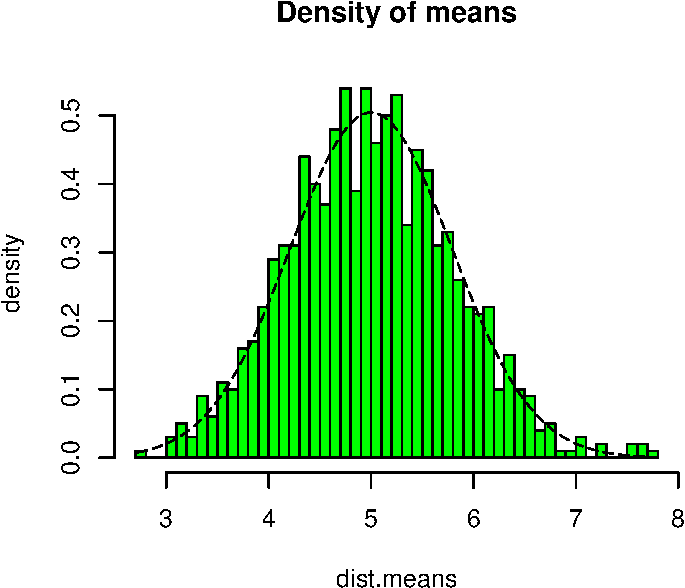
\includegraphics{./Q1_files/figure-latex/Q3.pdf}

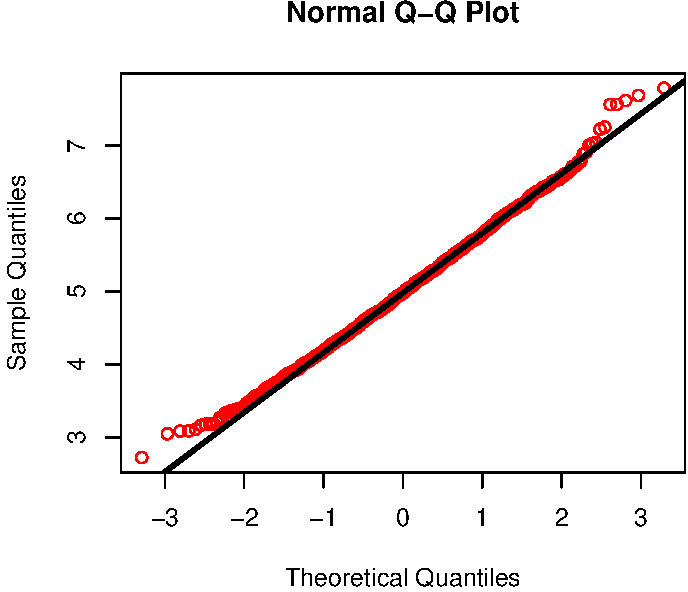
\includegraphics{./Q1_files/figure-latex/Q3_2.pdf}

In the first plot we have overlayed a normal distribution (in black)
over the density plot taken from the means of the exponential
distribution. To confirm the distribution we use a qqnorm plot and
overlay the theoretical line. We notice in the QQ plot that most of the
red is on the theoretical normal line and only deviates at the
begninning and end due to the skewness of the exponential distribution.

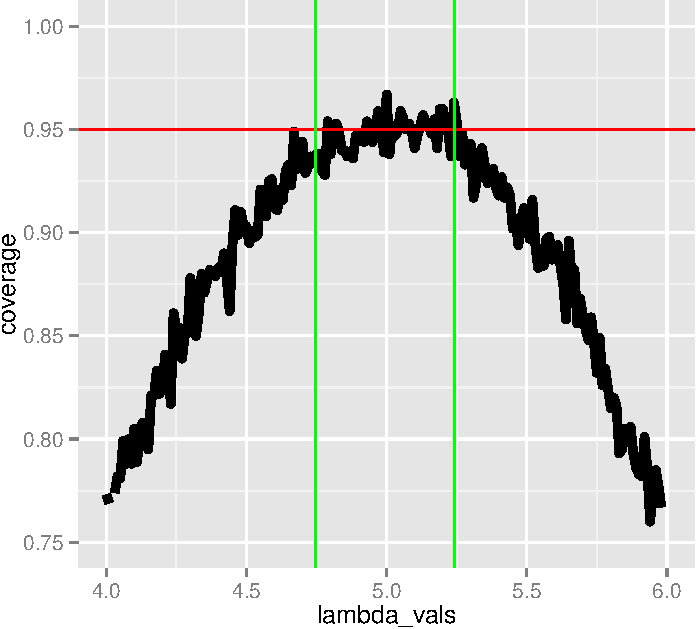
\includegraphics{./Q1_files/figure-latex/Q4.pdf} The interval above 95\%
is between 4.7476, 5.2426 and is depicted in the plot above using the
green lines. The red line shows the 95\% confidence interval line

The full report including all R code:
\href{}{\url{https://github.com/JacquesBot/StatisticalInference/blob/master/Q1.md}}

\end{document}
